% !TeX root = ../main.tex
% -*- coding: utf-8 -*-

\chapter{基于近边界数据的模型所有权推断方法研究}\label{4}

本章将从数据集推断引出近边界数据推断模型所有权的方法。

\section{理论驱动}\label{4.1}

\subsection{所有权验证局限性}

现有的模型知识产权保护措施着重于被动的防御,只考虑针对模型修改的抗攻击性。模型所有者将水印嵌入训练好的模型或从其中提取抽象的模型知识作为指纹(称为源模型),当怀疑一个模型(称为可疑模型)的知识来自于源模型,模型所有者可以利用水印或指纹被动地从外部验证模型所有权。大多数工作基于这样的思路,设计不同的水印和指纹用于在源模型被盗窃后验证模型所有权,但这并不具有较强的鲁棒性。模型水印的缺陷例如对源模型性能和功能的影响,嵌入水印引起的额外代价都是研究水印工作的关键点。模型指纹目的是提取代表模型知识的固有特征,相较于水印指纹不会对源模型产生影响,但是指纹是脆弱的因为模型知识是易被修改的,所有的指纹方法都试图找到可以承受某些修改攻击的强鲁棒性指纹。

本文的目标集中在水印和指纹另一个亟待解决的问题歧义攻击上,歧义攻击不关心如何去除水印和指纹以通过模型所有权验证,而是伪造额外的水印和指纹混淆所有权验证。具体来说,盗窃者对源模型嵌入新的水印或提取其他的指纹使本来的保护措施无效。歧义攻击对现有的深度神经网络模型的知识产权保护方法构成了严重威胁,在传统的数字水印领域中有研究表明,鲁棒性的水印可能不一定能验证所有权,除非水印方案是不可逆的\cite{fan2019rethinking}。在本文中,我们认为通过验证可疑模型是否具有源模型特定的水印或指纹来讨论盗窃行为是不充分的,特别是出现歧义攻击时,因此我们提出推断模型所有权而不是验证。这种方法的灵感来自于数据集推断\cite{maini2021dataset} 提出的所有权决策,我们将在\ref{4.1.2}中具体讨论。

\subsection{利用数据推断模型所有权}\label{4.1.2}

数据集推断做了一个假设:源模型的知识来自于训练数据集。无论盗窃模型是直接攻击源模型还是其副产品,盗窃模型的知识是源模型中包含的知识。如果原始训练数据集是私有的,模型所有者就比对手拥有强大优势,源模型在原始训练数据中的性能要远远优于其他数据集。因此,通过统计测试与估计多个数据点到决策边界的距离相结合,可以得到模型所有权归属。

源模型的知识被传播到盗窃模型使得所有盗窃模型都必须包含源模型训练数据集中的直接或间接信息。原始训练数据的私有性作为源模型的标识可以用来识别盗窃模型,只需要证明可疑模型和源模型都经过共同的私有数据集训练(不一定完全相同)。此过程和传统的验证模型所有权不同,通过私有数据集推断得到的是一个所有权决策,其中决策的最大者被认为拥有所有权。传统的模型所有权验证是从模型中提取水印或指纹进行匹配从而验证,这里涉及到了歧义攻击导致的验证冲突。 可以发现数据集推断得到的是一个“最”的概念,因此可以有效避免歧义攻击。因此,我们指出推断所有权将会成为未来模型知识产权保护技术的主要方向。

我们的工作受到数据集推理验证模型所有权的启发,我们提出了数据驱动推断所有权代替验证所有权。我们认为所有权推断在有效证明所有权归属问题的同时,可以解决验证冲突问题。除此之外,数据驱动的推断所有权意味着只和输入输出相关,我们的方法既可以在白盒环境也可以在黑盒环境下工作。

但是数据集推断具有以下\textbf{局限性}:
\begin{enumerate}
	\renewcommand{\labelenumi}{\theenumi)}
	\item 使用数据集推理的前提是原始训练数据不被盗窃者得到,公开数据集不能被用于训练源模型。然而,在大多数现实情况中,只有很少一部分工作会构造私有数据集用于训练模型,甚至这部分工作的应用点很狭窄,这意味着被盗窃的风险较小。因此,依赖于私有数据集的数据集推理方法在实际应用中使用范围很小,不能被大幅度推广使用;
	\item 数据集推理方法的核心思想是源模型的功能在训练数据上的效果优于其他数据,但存在模型的功能可能相似,而结构和训练数据都不同的情况。因此该方法可能会导致误导。Li等人\cite{lao2022deepauth}验证了此限制,结果表明该方法产生的结果值得怀疑。
\end{enumerate}

我们指出,利用数据推断所有权的想法需要解决以上问题,因此我们提出构造私有化近边界数据作为推断依据,并利用近边界数据靠近决策边界的特性处理模型功能相似引起的误导。这是因为即使模型功能相似,但决策边界不可能完全相同。

\section{近边界数据推断模型所有权}\label{4.2}

在本文中,我们提出了近边界数据,一种分布在分类边界附近的特殊样本。模型指纹\cite{cao2021ipguard}使用对抗性样本抽象地反映模型分类边界,同一组对抗性样本的输入,其引起的决策模式的变化可以用于比较模型知识的相似性,但这种方法是脆弱的,对模型的任意操作都有可能破坏这种特性。因此,我们不直接比较决策模式的变化,它是不可信任的,而是比较对抗性样本与决策边界的距离。有意思的是大多数对抗性样本都是位于决策边界附近的,也就是说,它们与决策边界的距离很近。对抗性样本的这种性质被我们所利用并构造近边界数据,经过测试我们发现绝大多数的模型窃取方法都无法改变这种结果,即使样本分类被影响,其仍然位于分类边界附近。近边界数据背后的意义是如果被用于所有权验证如果两个模型的决策模式相似,参与训练的近边界数据一定可以反映出来。受到这个的启发,将近边界数据作为水印验证所有权是传统的思路,即使不会对模型的精度造成影响,然而这样的水印是脆弱的,很难抵御歧义攻击,因此我们提出由近边界数据驱动的所有权推断方法,其思想是构造私有的近边界数据,当验证一个模型的所有权时,模型所有者和盗窃者分别提供各自的私有近边界数据,距离分类边界最近的被推断获得所有权。这个方法的主要思想如图\ref{方法原理图}所示。
\begin{figure}[htbp]%%图,[htbp]是浮动格式
	\centering
	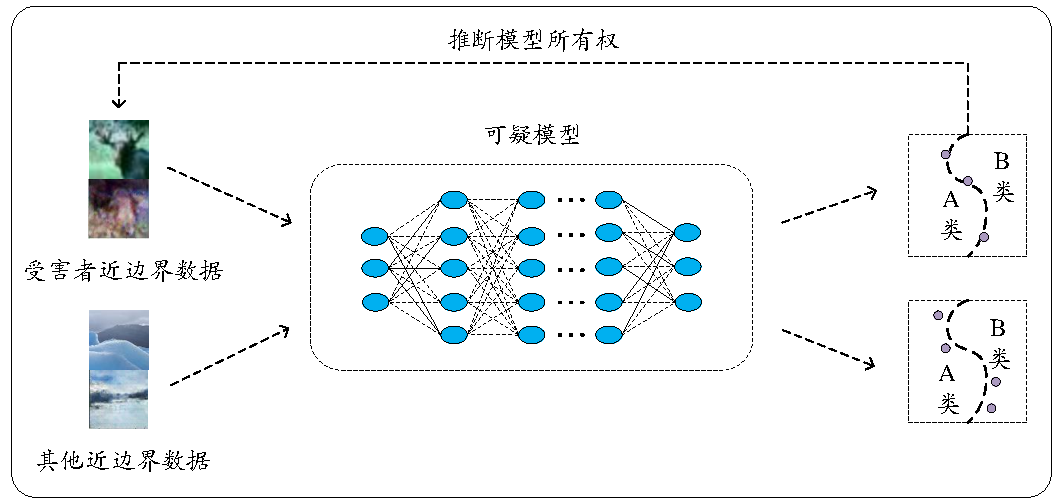
\includegraphics[width=14.5cm,height=7cm]{方法原理图.pdf}
%	\centerline{原始样本}
	\setlength{\abovecaptionskip}{5mm} %图片标题与图片距离
	\caption{近边界数据推断所有权}
	\label{方法原理图}
\end {figure}

\subsection{设计目标}

依据现有的工作,我们的方法在模型训练后进行部署,且在黑盒环境中推断所有权。我们的方法不关注模型盗窃的过程,目的是准确推断受害者所有权和识别可疑模型的盗窃行为。现在大多数所有权验证技术都是黑盒模型环境,因为模型所有者和攻击者通常不会提供完整模型。我们提出的方法仅利用模型提供的外部API,获取近边界数据的决策结果,从而推断模型所有权。在通常的假设中,存在一个官方的仲裁机构,当对任一模型产生所有权怀疑时,受害者和可疑对手可以向机构提出申请并提供各自的私有化近边界数据,并通过我们的方法推断所有权。注意无论在白盒和黑盒的环境中,我们的方法均可以产生效果。

为了实现推断模型所有权,本文提出的方法的设计目标是:
\begin{enumerate}
	\renewcommand{\labelenumi}{\theenumi)}
	\item \textbf{精确性:} 推断模型所有权的方法不应该影响模型的性能,模型的最大可接受测试精度下降不超过5\%。
	\item \textbf{数据近边界性:}如果可疑模型与源模型相同或来自源模型,则根据源模型构造的私有近边界数据在推断模型所有权中距离指定的分类边界最近。
	\item \textbf{鲁棒性:}近边界数据应该对常见的模型修改(如模型微调、剪枝和有损压缩)具有鲁棒性。
	\item \textbf{不可见性:}敌手无法获得私有的近边界数据,也无法在视觉上观察到近边界数据的部署。
	\item \textbf{有效性:}通过近边界数据推断模型所有权应能有效地计算距离边界数据,并通过对比全部近边界数据的决策结果确定可疑模型是盗窃模型。
\end{enumerate}

\subsection{方法概述}

为了实现以上目标,本文提出了一种基于近边界数据的模型所有权推断方法。

\noindent\textbf{问题定义:}我们定义了一个深度神经网络(DNN)分类器$G$作为源模型,给定一个原始训练集$D$,假设该源模型是一个$n$-类的DNN分类器,分类器的输出层为softmax层或其他决策层,决策函数$g_j(x)$表示数据样本$x$被分到第$j$类的概率,其中$j$ = 1,2,..,$n$。$Z_1$,$Z_2$,..,$Z_n$表示模型分类器的全部决策函数输出,其结果可作为分类边界的依据被我们使用,因此

\begin{equation}
	g_j(x) = \frac{exp(Z_j(x))}{\sum_{i = 1}^n exp(Z_i(x))}
\end{equation}

\noindent 其中,数据样本$x$的标签$y$被推断拥有最大概率的类别,例如$y = arg \mathop{max} \limits_j g_j(x) = arg \mathop{max} \limits_j Z_j(x)$。

\begin{myDef}
	\label{def:2}
	\pmb{分类边界}。分类器的分类边界是一个抽象的概念,我们无法直接描述它。因此我们使用分类器的决策结果来反映分类边界。
\end{myDef}

通常来说,寻找位于分类边界上的数据点采用重复随机采样数据点的方法,具体地如果数据点满足上述定义则数据点在分类边界上。然而,简单的重复采样可能需要大量的时间消耗,甚至无法找到这样的数据点们。为了解决这样的问题,我们在\ref{3}中讨论了如何构造位于分类边界上或其附近的的数据点,且将其私有化的过程。

基于\ref{3}的讨论,我们提出构造近边界数据推断模型的所有权,而不是验证所有权。具体而言,如图\ref{方法流程图}所示,我们的方法包括三个主要阶段:
\begin{enumerate}
	\renewcommand{\labelenumi}{\theenumi)}
	\item 从数据集样本中生成对抗性样本;
	\item 训练生成对抗模型生成私有化的近边界数据;
	\item 加入近边界数据微调源模型。
\end{enumerate}

\begin{figure}[htbp]%%图,[htbp]是浮动格式
	\centering
	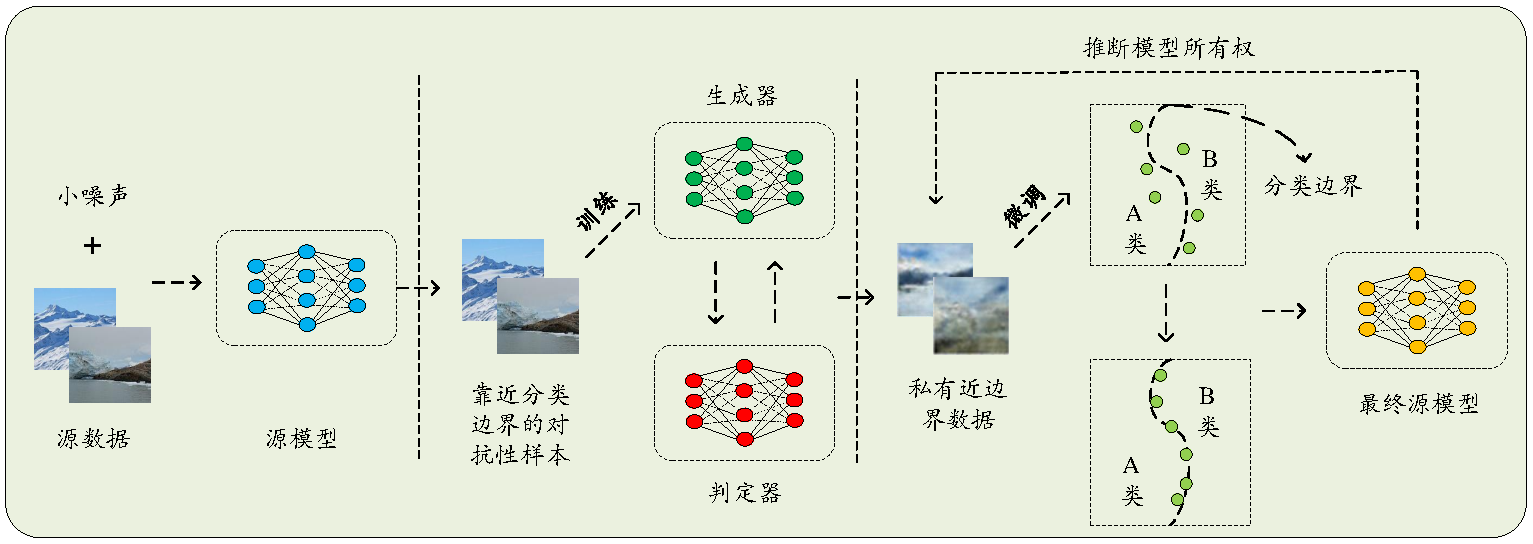
\includegraphics[width=14.5cm,height=7cm]{方法流程图.pdf}
	%	\centerline{原始样本}
	\setlength{\abovecaptionskip}{5mm} %图片标题与图片距离
	\caption{方法整体流程图}
	\label{方法流程图}
\end {figure}

\subsection{假设检验}\label{4.2.3}

根据\ref{4}\ref{4.1}讨论的结果,本文认为过去的验证模型所有权的思路具有较大的局限性,大多数研究无法抵御歧义攻击。因此,我们提出了推断模型所有权的想法,这是一种“最”的思路。在现实情况中,我们假设存在第三方仲裁机构,并约定目标分类边界,被盗窃者向第三方机构提出仲裁并提供近边界数据,盗窃者同样需要提供相应的近边界数据,第三方机构分别计算目标分类边
界距离,本文认为持有最靠近目标分类边界的近边界数据所有者将获得模型所有权。注意由于近边界数据通常是一组数据,所以应该根据统计的结果来看。在实践中,我们计算了不同规模的近边界数据组在源模型, 盗窃模型和不相关模型上与分类边界的距离,并设计了一种基于假设检验的方法来表现推断置信度。

\noindent\textbf{假设检验:}我们假设事件$C$是模型所有者提供的私有近边界数据在怀疑模型上的计算结果,事件$C_S$ 表示盗窃者提供的近边界数据在怀疑模型上的计算结果,或模型所有者提供的私有近边界数据在无关模型上的计算结果。本文计算假设$H_0:\mu > \mu_S(H_1:\mu\leq\mu_S)$的$p$值,以及差异大小$\Delta \mu = \mu_S - \mu$,$\Delta\mu$越大,推断可信度越高。如果$p$值低于预定义的置信度评分$\alpha$,则拒绝$H_0$,并称正在测试的模型是被盗模型。我们重复30次统计性实验以提高可信度。


\begin{algorithm}[htbp]
	\setstretch{1.2}
	\caption{InitialDistribution}
	\label{alg:1}
	\begin{algorithmic}[1]
		
		\Require $Nodes,kFrags,Set$
		\Ensure $targetnodes$
		\State $Nodes \gets$ the neighboring online nodes
		\State $kFrags \gets$ the N re-encryption keys the node has generated
		\State $Set \gets$ the set of the nodes that have got the kFrag
		\State $flag \gets$ 0
		\For {$kFrag$ in $kFrags$}
		\State
		\Call{SelectNode}{$Nodes,kFrag,Set,underload$}
		\If{$flag==0$}
		\State \Call{SelectNode}{$Nodes,kFrag,Set,normal$}
		\EndIf
		\If{$flag==0$}
		\State \Call{SelectNode}{$Nodes,kFrag,Set,overload$}
		\EndIf
		\EndFor
		
		
		\State    
		\Function{SelectNode}{$Nodes,kFrag,Set,State$}
		\For{$node$ in $Nodes$}
		\If {$node's$ $state$ is $State$ and $node$ $\notin$ $Set$}
		\State $Send(kFrag)$
		\State $Set=Set \cup node$
		\If{$Size(Set)==Size(Map)$}
		\State $Clear(Set)$
		\EndIf
		\State $flag \gets 1$
		\State $Break$
		
		
		\EndIf
		\EndFor
		\EndFunction
		
		
	\end{algorithmic}
\end{algorithm}

\section{本章小结}

本章从所有权验证的局限性出发,引出了数据集推断,然后详细介绍了近边界数据推断模型所有权的设计目标以及具体的方法流程。

